\documentclass[letterpaper,10pt]{article}
\usepackage[top=2cm, bottom=1.5cm, left=1cm, right=1cm]{geometry}
\usepackage{amsmath, amssymb, amsthm,graphicx, enumitem}
\usepackage{fancyhdr}
\pagestyle{fancy}

\lhead{\today}
\chead{MultiVariate Stats Assignment 4}
\rhead{Justin Hood}

\newcommand{\Z}{\mathbb{Z}}
\newcommand{\Q}{\mathbb{Q}}
\newcommand{\R}{\mathbb{R}}
\newcommand{\C}{\mathbb{C}}
\newtheorem{lem}{Lemma}

\begin{document}
\begin{description}
\item[4.6]\hfill\\
Let $\textbf{X}$ be distributed as $N_3(\mu,\Sigma)$ where $\mu'=[1,-1,2]$. And,
\[\Sigma=\begin{bmatrix}
4 & 0 & -1\\0 & 5 & 0\\-1 & 0 & 2
\end{bmatrix} \]
Given that $\Sigma$ is the Variance-Covariance matrix of $\textbf{X}$, we consider the following cases,
\begin{enumerate}[label=\alph*.]
\item $X_1$ and $X_2$\\
Consulting the $\Sigma$ matrix, we find,
\[Cov(X_1,\ X_2)=\sigma_{12}=0\]
Thus, we see that these variables are independent of each other.
\item $X_1$ and $X_3$\\
Again, we compute,
\[Cov(X_1,\ X_3)=\sigma_{13}=-1\]
Hence, we see that these variables are not independent of eachother.
\item $X_2$ and $X_3$\\
Again,
\[Cov(X_2,\ X_3)=\sigma_{23}=0\]
Thus, we see that these variables are independent.
\item $(X_1,\ X_3)$ and $X_2$\\
We shall now convert our $\Sigma$ matrix such that we can compare the $(X_1,\ X_3)$ and $X_2$. Here,
\[\Sigma \to \left[\begin{tabular}{cc|c}
4 & 1 & 0\\
-1 & 2 & 0\\\hline
0 & 0 & 5
\end{tabular} \right] \]
A ``2x2" matrix for comparison. Then, we have,
\[Cov((X_1,\ X_3),\ X_2)=\begin{bmatrix}
0\\0
\end{bmatrix}\]
Which from the text, we see is independent.
\item $X_1$ and $X_1+3X_2-2X_3$\\
We see that the covariance can be computed as,
\[Cov(X_1,\ X_1+3X_2-2X_3)=\sigma_{11}+3\sigma_{12}-2\sigma_{13}=6\]
Thus, they are not independent.
\end{enumerate}
\item[4.7]\hfill\\
\begin{enumerate}[label=\alph*.]
\item Compute the conditional distribution of $X_1$, given $X_3=x_3$.\\
We consider the joint distribution of $(X_1,\ X_3)$ is,
\[(X_1,\ X_3)\sim N_2\left(\begin{bmatrix}
\mu_1\\ \mu_3
\end{bmatrix}, \begin{bmatrix}
\Sigma_{11} & \Sigma_{13}\\\Sigma_{31} & \Sigma_{33}
\end{bmatrix} \right)\]
Thus, the conditional distribution of $f(X_1|X_3=x_3)$ becomes,
\begin{align*}
f(X_1|X_3=x_3) &\sim N\left(\mu_1+\frac{\sigma_{13}}{\sigma_{33}}(x_3-\mu_3),\ \sigma_{11}-\frac{\sigma_{13}^2}{\sigma_{33}}\right)\\
&\sim N\left(1+\frac{-1}{2}(x_3-2),\ 4-\frac{(-1)^2}{2}\right)\\
&\sim N(1-.5(x_3-2),\ 3.5)
\end{align*}
\item Similarly,
\begin{align*}
f(X_1|X_2=x_2,X_3=x_3) &\sim N\left(\mu_1+\frac{\sigma_{13}}{\sigma_{33}}(x_3-\mu_3)+\frac{\sigma_{12}}{\sigma_{22}}(x_2-\mu_2),\ \sigma_{11}-\frac{\sigma_{13}^2}{\sigma_{33}}-\frac{\sigma_{12}^2}{\sigma_{22}}\right)\\
&\sim N\left(1+\frac{-1}{2}(x_3-2)+\frac{0}{5}(x_2+1),\ 4-\frac{(-1)^2}{2}-\frac{0^2}{5}\right)\\
&\sim N(1-.5(x_3-2),\ 3.5)
\end{align*}
The same as in part a. We see that this is due to the fact that the covariance is 0 for $X_1$ and $X_2$.
\end{enumerate}
\item[4.17]\hfill\\
Let $\textbf{X}_1,\textbf{X}_2,\textbf{X}_3,\textbf{X}_4,\textbf{X}_5$ be independent and identically distributed random vectors with mean vector $\mu$ and covariance matrix $\Sigma$. Consider now the mean and covariances of,
\begin{enumerate}[label=\alph*.]
\item $V_1=\sum_i\frac{1}{5}\textbf{X}_i$\\
The mean and covariance of this vector is given by,
\[V_1\sim N\left(\sum_{i=1}^{5}a_i\mu_i, \left(\sum_{i=1}^{5}a_i^2\right)\Sigma\right),\ a_i=\frac{1}{5}\]
So,
\begin{align*}
\mu(V_1) &= \sum_{i=1}^5a_i\mu_i && \text{Given that }\mu_i\text{ are identical}\\
&=\mu\sum_{i=1}^5\frac{1}{5}\\
&=\mu
\end{align*}
and,
\begin{align*}
Cov(V_1) &= \left(\sum_{i=1}^{5}a_i^2\right)\Sigma && \text{Similarly to before, we factor }\Sigma\\
&=\Sigma \sum_{i=1}^5\frac{1}{5^2}\\
&=\frac{\Sigma}{5}
\end{align*}
\item $V_2=\textbf{X}_1-\textbf{X}_2+\textbf{X}_3-\textbf{X}_4+\textbf{X}_5$\\
As before,
\begin{align*}
\mu(V_2) &=\sum_{i=1}^5c_i\mu_i && \text{Given that }\mu_i\text{ are identical}\\
&=\mu\sum_{i=1}^5c_i\\
&=\mu(1-1+1-1+1)\\
&=\mu
\end{align*}
And,
\begin{align*}
Cov(V_2) &= \left(\sum_{i=1}^5c_i^2\right)\Sigma && \text{Similarly to before, we factor }\Sigma\\
&=\Sigma(1+1+1+1+1)\\
&=5\Sigma
\end{align*}
\item Finally, we consider the covariance between the two vectors as,
\[\begin{bmatrix}
V_1\\V_2
\end{bmatrix}\sim N\left(\begin{bmatrix}
\mu \\ \mu
\end{bmatrix}, \Sigma^*\right) \]
Where,
\[\Sigma^*=\begin{bmatrix}
(\sum a_i^2)\Sigma & (a'c)\Sigma\\\\
(a'c)\Sigma & (\sum c_i^2)\Sigma
\end{bmatrix}=\begin{bmatrix}
\frac{1}{5}\Sigma & \frac{1}{5}\Sigma\\\\
\frac{1}{5}\Sigma & 5\Sigma
\end{bmatrix} \]
\end{enumerate}
\item[4.18]\hfill\\
Consider,
\[\textbf{X}=\begin{bmatrix}
3 & 6\\4 & 4\\5 & 7\\4 & 7
\end{bmatrix} \]
To find the maximum likelihood estimates of $\mu$ and $\Sigma$ we use the equations,
\begin{align*}
\hat{\mu} &= \bar{\textbf{X}}\\
\hat{\Sigma} &= \frac{1}{n}\sum_{j=1}^n(X_j-\bar{X})(X_j-\bar{X})'
\end{align*}
Using $R$, we easily compute both values to be,
\begin{align*}
\hat{\mu} &=[4,\ 6]\\
\hat{\Sigma} &= \frac{1}{4}\begin{bmatrix}
2 & 1\\1 & 6
\end{bmatrix}
\end{align*}
\item[4.19]\hfill\\
Let $\textbf{X}_1,\ \textbf{X}_2,\ \ldots,\ \textbf{X}_{20}$ be a random sample of size $n=20$ from a $N_6(\mu,\Sigma)$ population. We consider the following,
\begin{enumerate}[label=\alph*.]
\item Distribution of $(\textbf{X}_1-\mu)'\Sigma^{-1}(\textbf{X}_1-\mu)$.\\
Consider from the text, Result 4-7. Given a measurement $\textbf{X}$ distributed $N_p(\mu,\Sigma)$, then, $(\textbf{X}-\mu)'\Sigma^{-1}(\textbf{X}-\mu)\sim \chi_p^2$ Thus, we can consider the distribution to be,
\[(\textbf{X}_1-\mu)'\Sigma^{-1}(\textbf{X}_1-\mu)\sim\chi_6^2 \]
\item Distribution of $\bar{\textbf{X}}$ and $\sqrt{n}(\bar{\textbf{X}}-\mu)$.\\
Consider first, $\bar{\textbf{X}}$. From the text, we see that box 4-23 tells us that
\[\bar{\textbf{X}}\sim N_p(\mu,(1/n)\Sigma)=N_6(\mu,\frac{1}{20}\Sigma)\]
Similarly, we may now consider, $\sqrt{n}(\bar{\textbf{X}}-\mu)$. Box 4-28 tells us that,
\[\sqrt{n}(\bar{\textbf{X}}-\mu)\sim N_p(0,\Sigma)=N_6(0,\Sigma)\]
This makes sense, given the structure of the distribution of $\bar{\textbf{X}}$. Shifting by $\mu$ will reduce the mean, and scaling by $\sqrt{n}$ will scale the covariance appropriately.
\item Distribution of $(n-1)\textbf{S}$. From box 4-23, we see that this is distributed as a Wishart random matrix with $(n-1)$ degrees of freedom. So,
\[(n-1)S\sim W_{19}(\ \boldsymbol{\cdot}\ |\Sigma)\]
\end{enumerate}
\item[4.25]\hfill \\
We consider the data from problem 1.4. Using all three variables and the quantile cuttoffs, \[<0.3518,.7978,1.2125,1.6416,2.1095,2.6430,3.2831,4.1083,5.317,7.8147>\]
We construct the chi-square plot of all three variables with the cuttofs above, shown below,
\begin{center}
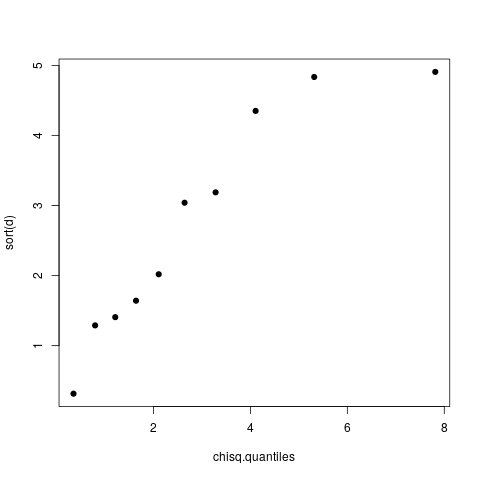
\includegraphics[scale=.75]{425.png}
\end{center}
\item[4.29]\hfill\\
We consider the data from Table 1.5 specifically the pairs from $X_5=NO_2$ and $X_6=O_3$. We consider the follow,
\begin{enumerate}[label=\alph*.]
\item Compute the statistical distances $(x_j-\bar{x})S^{-1}(x_j-\bar{x})$.\\
The distances are,\\
$<0.4606524, 0.6592206,  2.3770610,  1.6282902,  0.4135364, 0.4760726,  1.1848895, 10.6391792,  0.1388339,  0.8162468,\\
1.3566301,  0.6228096,  5.6494392,  0.3159498,  0.4135364, 0.1224973,  0.8987982,  4.7646873,  3.0089122,  0.6592206,\\
2.7741416,  1.0360061,  0.7874152,  3.4437748,  6.1488606, 1.0360061,  0.1388339,  0.8856041,  0.1379719,  2.2488867,\\
0.1901188,  0.4606524,  1.1471939,  7.0857237,  1.4584229, 0.1224973,  1.8984708,  2.7782596,  8.4730649,  0.6370218,\\
0.7032485,  1.8013611$
This data is more concisely contained in the attached $R$ code as well under the variable $d$ in section 4.29.
\item The cutoff for a bivariate normal distribution with a $.5$ probability contour is $1.38629$. For this data, we have that $0.6190476$ of the data falls within the 50\% contour.
\item The Chi-Squared plot of the data from $a$ is shown below,
\begin{center}
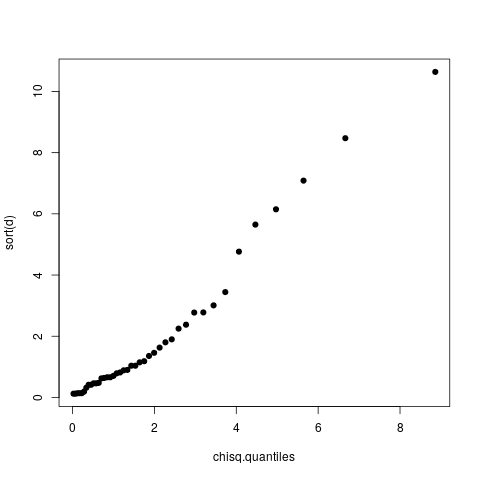
\includegraphics[scale=.75]{429.png}
\end{center}
\end{enumerate}
\end{description}
\end{document}
